\documentclass[12pt]{article}
\usepackage{fancyvrb,amsmath,amsfonts,amssymb,graphicx,listings}
\usepackage[usenames,dvipsnames,svgnames,table]{xcolor}
%\usepackage{parskip}
\usepackage{slashed}
\usepackage{tikz}
\usepackage{mathrsfs}

% change margins
\addtolength{\oddsidemargin}{-.875in}
\addtolength{\evensidemargin}{-.875in}
\addtolength{\textwidth}{1.75in}
\addtolength{\topmargin}{-.875in}
\addtolength{\textheight}{1.75in}

\hyphenpenalty=10000

\begin{document}

\begin{center}
{\sc electron positron annihilation}
\end{center}

\noindent
Electron positron annihilation creates two photons.
\begin{center}
\begin{tikzpicture}
\draw[dashed] (0,0) circle (0.5cm);
\draw[thick,->] (2,0) node[anchor=west] {$e^+$} -- (0.6,0);
\draw[thick,->] (-2,0) node[anchor=east] {$e^-$} -- (-0.6,0);
\draw[thick,->] (0.40,0.40) -- (1.3,1.3) node[anchor=south west] {$\gamma$};
\draw[thick,->] (-0.4,-0.4) -- (-1.3,-1.3) node[anchor=north east] {$\gamma$};
\draw (1,0.5) node {$\theta$};
\end{tikzpicture}
\end{center}

\noindent
Here is the same diagram with momentum and spinor labels.
\begin{center}
\begin{tikzpicture}
\draw[dashed] (0,0) circle (0.5cm);
\draw[thick,->] (2,0) node[anchor=west] {$p_2, v_2$} -- (0.6,0);
\draw[thick,->] (-2,0) node[anchor=east] {$p_1, u_1$} -- (-0.6,0);
\draw[thick,->] (0.40,0.40) -- (1.3,1.3) node[anchor=south west] {$p_3$};
\draw[thick,->] (-0.4,-0.4) -- (-1.3,-1.3) node[anchor=north east] {$p_4$};
\draw (1,0.5) node {$\theta$};
\end{tikzpicture}
\end{center}

\noindent
In a typical collider experiment the momentum vectors are
\begin{equation*}
p_1=\begin{pmatrix}E\\0\\0\\p\end{pmatrix}
\qquad
p_2=\begin{pmatrix}E\\0\\0\\-p\end{pmatrix}
\qquad
p_3=\begin{pmatrix}E\\ E\sin\theta\cos\phi\\ E\sin\theta\sin\phi\\ E\cos\theta\end{pmatrix}
\qquad
p_4=\begin{pmatrix}E\\ -E\sin\theta\cos\phi\\ -E\sin\theta\sin\phi\\ -E\cos\theta\end{pmatrix}
\end{equation*}

\noindent
where $E=\sqrt{p^2+m^2}$.

\bigskip
\noindent
The spinors are
\begin{equation*}
\underset{\text{inbound electron, spin up}}
{u_{11}=\begin{pmatrix}E+m\\0\\p\\0\end{pmatrix}}
\qquad
\underset{\text{inbound electron, spin down}}
{u_{12}=\begin{pmatrix}0\\E+m\\0\\-p\end{pmatrix}}
\qquad
\underset{\text{inbound positron, spin up}}
{v_{21}=\begin{pmatrix}-p\\0\\E+m\\0\end{pmatrix}}
\qquad
\underset{\text{inbound positron, spin down}}
{v_{22}=\begin{pmatrix}0\\p\\0\\E+m\end{pmatrix}}
\end{equation*}

\noindent
The spinors shown above are not individually normalized.
Instead, a combined spinor normalization constant $N=(E+m)^2$ will be used.

\bigskip
\noindent
The following formula computes a probability density $|\mathcal{M}_{ab}|^2$
for annihilation where $a$ is the spin state of the inbound electron and
$b$ is the spin state of the inbound positron.
The formula is from Feynman diagrams.
\begin{equation*}
|\mathcal{M}_{ab}|^2
=
\frac{e^4}{N}
\left|
-\frac{\bar{v}_{2b}\gamma^\mu(\slashed{q}_1+m)\gamma^\nu u_{1a}}{t-m^2}
-\frac{\bar{v}_{2b}\gamma^\nu(\slashed{q}_2+m)\gamma^\mu u_{1a}}{u-m^2}
\right|^2
\end{equation*}

\noindent
Symbol $e$ is electron charge.
Symbol $q_1=p_1-p_3$ and $q_2=p_1-p_4$.
Symbols $t$ and $u$ are Mandelstam variables $t=(p_1-p_3)^2=q_1^2$ and $u=(p_1-p_4)^2=q_2^2$.

\bigskip
\noindent
Let
\begin{equation*}
a_1=\bar{v}_{2b}\gamma^\mu(\slashed{q}_1+m)\gamma^\nu u_{1a}
\qquad
a_2=\bar{v}_{2b}\gamma^\nu(\slashed{q}_2+m)\gamma^\mu u_{1a}
\end{equation*}

\noindent
Then
\begin{align*}
|\mathcal{M}_{ab}|^2&=\frac{e^4}{N}\left|-\frac{a_1}{t-m^2}-\frac{a_2}{u-m^2}\right|^2\\
&=
\frac{e^4}{N}
\left(-\frac{a_1}{t-m^2}-\frac{a_2}{u-m^2}\right)
\left(-\frac{a_1}{t-m^2}-\frac{a_2}{u-m^2}\right)^*\\
&=
\frac{e^4}{N}\left(
\frac{a_1a_1^*}{(t-m^2)^2}
+\frac{a_1a_2^*}{(t-m^2)(u-m^2)}
+\frac{a_1^*a_2}{(t-m^2)(u-m^2)}
+\frac{a_2a_2^*}{(u-m^2)^2}
\right)
\end{align*}

\noindent
The expected probability density $\langle|\mathcal{M}|^2\rangle$
is computed by summing $|\mathcal{M}_{ab}|^2$ over all spin and polarization states
and then dividing by the number of inbound states.
There are four inbound states.
The sum over polarization states is already accomplished by contraction
of $aa^*$ over $\mu$ and $\nu$.
\begin{align*}
\langle|\mathcal{M}|^2\rangle
&=\frac{1}{4}\sum_{a=1}^2\sum_{b=1}^2|\mathcal{M}_{ab}|^2\\
&=\frac{e^4}{4N}\sum_{a=1}^2\sum_{b=1}^2
\left(
\frac{a_1a_1^*}{(t-m^2)^2}
+\frac{a_1a_2^*}{(t-m^2)(u-m^2)}
+\frac{a_1^*a_2}{(t-m^2)(u-m^2)}
+\frac{a_2a_2^*}{(u-m^2)^2}
\right)
\end{align*}

\noindent
Use the Casimir trick to replace sums over spins with matrix products.
\begin{align*}
f_{11}&=\frac{1}{N} \sum_{a=1}^2\sum_{b=1}^2 a_1a_1^*=\mathop{\rm Tr}
\left(
(\slashed{p}_1+m)\gamma^\mu(\slashed{q}_1+m)\gamma^\nu(\slashed{p}_2-m)\gamma_\nu(\slashed{q}_1+m)\gamma_\mu
\right)
\\
f_{12}&=\frac{1}{N} \sum_{a=1}^2\sum_{b=1}^2 a_1a_2^*=\mathop{\rm Tr}
\left(
(\slashed{p}_1+m)\gamma^\mu(\slashed{q}_2+m)\gamma^\nu(\slashed{p}_2-m)\gamma_\mu(\slashed{q}_1+m)\gamma_\nu
\right)
\\
f_{22}&=\frac{1}{N} \sum_{a=1}^2\sum_{b=1}^2 a_2a_2^*=\mathop{\rm Tr}
\left(
(\slashed{p}_1+m)\gamma^\mu(\slashed{q}_2+m)\gamma^\nu(\slashed{p}_2-m)\gamma_\nu(\slashed{q}_2+m)\gamma_\mu
\right)
\end{align*}

\noindent
Hence
\begin{equation*}
\langle|\mathcal{M}|^2\rangle
=
\frac{e^4}{4}
\left(
\frac{f_{11}}{(t-m^2)^2}
+\frac{f_{12}}{(t-m^2)(u-m^2)}
+\frac{f_{12}^*}{(t-m^2)(u-m^2)}
+\frac{f_{22}}{(u-m^2)^2}
\right)
\end{equation*}

\noindent
Run ``annihilation-1.txt'' to verify the Casimir trick for electron positron annihilation.

\bigskip
\noindent
The following momentum formulas are equivalent to the Casimir trick.
(Recall that $a\cdot b=a^\mu g_{\mu\nu}b^\nu$)
\begin{align*}
f_{11}&=
16 (p_1 \cdot p_1) (p_1 \cdot p_2) -
32 (p_1 \cdot p_1) (p_2 \cdot p_3) -
16 (p_1 \cdot p_2) (p_3 \cdot p_3) +
32 (p_1 \cdot p_3) (p_2 \cdot p_3) %-
\\&\phantom{=}\qquad{}-
48 m^2 (p_1 \cdot p_2) +
64 m^2 (p_1 \cdot p_3) +
64 m^2 (p_2 \cdot p_3) -
64 m^2 (p_3 \cdot p_3) - 64 m^4
\\
f_{12}&=
-32 (p_1 \cdot p_1) (p_1 \cdot p_2) +
 32 (p_1 \cdot p_2) (p_1 \cdot p_3) +
 32 (p_1 \cdot p_2) (p_1 \cdot p_4) -
 32 (p_1 \cdot p_2) (p_3 \cdot p_4) %-
\\&\phantom{=}\qquad{}-
 48 m^2 (p_1 \cdot p_1) +
 48 m^2 (p_1 \cdot p_2) +
 32 m^2 (p_1 \cdot p_3) +
 32 m^2 (p_1 \cdot p_4) %-
\\&\phantom{=}\qquad{}-
 16 m^2 (p_2 \cdot p_3) -
 16 m^2 (p_2 \cdot p_4) -
 16 m^2 (p_3 \cdot p_4) + 32 m^4
\\
f_{22}&=
16 (p_1 \cdot p_1) (p_1 \cdot p_2) -
32 (p_1 \cdot p_1) (p_2 \cdot p_4) -
16 (p_1 \cdot p_2) (p_4 \cdot p_4) +
32 (p_1 \cdot p_4) (p_2 \cdot p_4) %-
\\&\phantom{=}\qquad{}-
48 m^2 (p_1 \cdot p_2) +
64 m^2 (p_1 \cdot p_4) +
64 m^2 (p_2 \cdot p_4) -
64 m^2 (p_4 \cdot p_4) - 64 m^4
\end{align*}

\noindent
In Mandelstam variables $s=(p_1+p_2)^2$, $t=(p_1-p_3)^2$, $u=(p_1-p_4)^2$ the formulas are
\begin{align*}
f_{11}&=8 t u - 24 t m^2 - 8 u m^2 - 8 m^4
\\
f_{12}&=8 s m^2 - 32 m^4
\\
f_{22}&=8 t u - 8 t m^2 - 24 u m^2 - 8 m^4
\end{align*}

\noindent
When $E\gg m$ a useful approximation is to set $m=0$ and obtain
\begin{align*}
f_{11}&=8tu
\\
f_{12}&=0
\\
f_{22}&=8tu
\end{align*}

\noindent
For $m=0$ the Mandelstam variables are
\begin{align*}
s&=4E^2\\
t&=-2E^2(1-\cos\theta) = -4 E^2 \sin^2(\theta/2)\\
u&=-2E^2(1+\cos\theta) = -4 E^2 \cos^2(\theta/2)
\end{align*}

\noindent
The corresponding expected probability density is
\begin{align*}
\langle|\mathcal{M}|^2\rangle
&=
\frac{e^4}{4}
\left(
\frac{8tu}{t^2}
+
\frac{8tu}{u^2}
\right)
\\
&=2e^4\left(\frac{u}{t}+\frac{t}{u}\right)
\\
&=2e^4\left(
\frac{1+\cos\theta}{1-\cos\theta}+
\frac{1-\cos\theta}{1+\cos\theta}
\right)
\end{align*}

\noindent
Substituting $e^4=16\pi^2\alpha^2$ we have
\begin{equation*}
\langle|\mathcal{M}|^2\rangle
=32\pi^2\alpha^2\left(
\frac{1+\cos\theta}{1-\cos\theta}+
\frac{1-\cos\theta}{1+\cos\theta}
\right)
\end{equation*}

\noindent
The resulting differential cross section is
\begin{equation*}
\frac{d\sigma}{d\Omega}=\frac{\langle|\mathcal{M}|^2\rangle}{64\pi^2s}
=\frac{\alpha^2}{8E^2}\left(
\frac{1+\cos\theta}{1-\cos\theta}+
\frac{1-\cos\theta}{1+\cos\theta}
\right)
\end{equation*}

\noindent
Run ``annihilation-2.txt'' to verify.

\bigskip
\noindent
We can integrate $d\sigma$ to obtain a cumulative distribution function.
Recall that
\begin{equation*}
d\Omega=\sin\theta\,d\theta\,d\phi
\end{equation*}

\noindent
Hence
\begin{equation*}
d\sigma=
\frac{\alpha^2}{8E^2}
\left(
\frac{1+\cos\theta}{1-\cos\theta}+
\frac{1-\cos\theta}{1+\cos\theta}
\right)\sin\theta\,d\theta\,d\phi
\end{equation*}

\noindent
Let $I(\theta)$ be the following integral of $d\sigma$.
\begin{align*}
I(\theta)&=
\left(\frac{8E^2}{\alpha^2}\right)\frac{1}{2\pi}
\int_0^{2\pi}\int d\sigma
\\
&=\int
\left(
\frac{1+\cos\theta}{1-\cos\theta}+
\frac{1-\cos\theta}{1+\cos\theta}
\right)
\sin\theta\,d\theta,
\quad a\le\theta\le\pi-a
\end{align*}

\noindent
Angular support is limited to an arbitrary $a>0$
because $I(0)$ and $I(\pi)$ are undefined.

\bigskip
\noindent
Let $C$ be the normalization constant
\begin{equation*}
C=I(\pi-a)-I(a)
\end{equation*}

\noindent
Then the cumulative distribution function $F(\theta)$ is
\begin{equation*}
F(\theta)=\frac{I(\theta)-I(a)}{C},
\quad a\le\theta\le\pi-a
\end{equation*}

\noindent
The probability of observing scattering events in the interval
$\theta_1$ to $\theta_2$ can now be computed.
\begin{equation*}
P(\theta_1\le\theta\le\theta_2)=F(\theta_2)-F(\theta_1)
\end{equation*}

\noindent
Probability density function $f(\theta)$ is the derivative of $F(\theta)$.
\begin{equation*}
f(\theta)=\frac{dF(\theta)}{d\theta}=\frac{1}{C}
\left(
\frac{1+\cos\theta}{1-\cos\theta}+
\frac{1-\cos\theta}{1+\cos\theta}
\right)\sin\theta,
\quad a\le\theta\le\pi-a
\end{equation*}

\noindent
Run ``annihilation-4.txt" to plot $f(\theta)$ for $a=\pi/6=30^\circ$.

\begin{center}
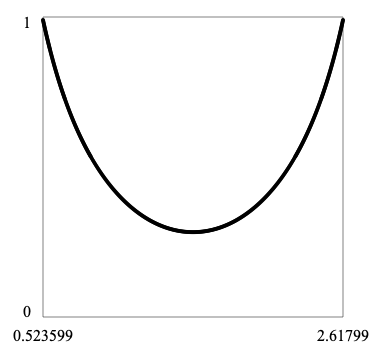
\includegraphics[scale=0.5]{annihilation.png}
\end{center}

\noindent
This is the probability distribution for $30^\circ$ bins and $a=30^\circ$.

\begin{center}
\begin{tabular}{|c|c|c|}
\hline
$\theta_1$ & $\theta_2$ & $P(\theta_1\le\theta\le\theta_2)$\\
\hline
$0^\circ$ & $30^\circ$ & -- \\
$30^\circ$ & $60^\circ$ & 0.33 \\
$60^\circ$ & $90^\circ$ & 0.17 \\
$90^\circ$ & $120^\circ$ & 0.17 \\
$120^\circ$ & $150^\circ$ & 0.33 \\
$150^\circ$ & $180^\circ$ & -- \\
\hline
\end{tabular}
\end{center}

\newpage
\noindent
The following table shows DESY-PETRA electron positron annihilation
data.\footnote{{\tt www.hepdata.net/record/ins191231} (Table 2, 14.0 GeV)}

\begin{center}
\begin{tabular}{|c|c|}
\hline
$x$ & $y$\\
\hline
$0.0502$ & 0.09983\\
$0.1505$ & 0.10791\\
$0.2509$ & 0.12026\\
$0.3512$ & 0.13002\\
$0.4516$ & 0.17681\\
$0.5521$ & 0.1957\phantom{0}\\
$0.6526$ & 0.279\phantom{00}\\
$0.7312$ & 0.33204\\
\hline
\end{tabular}
\end{center}

\noindent
Data $x$ and $y$ have the following relationship
with the differential cross section formula.
\begin{equation*}
x=\cos\theta
\qquad
y=\frac{d\sigma}{d\Omega}
\end{equation*}

\noindent
To compute predicted values $\hat{y}$ from the cross section formula,
use $\sqrt{s}=2E=14.0\,\text{GeV}$.
Multiply by $(\hbar c)^2$ to convert to SI
and multiply by $10^{37}$ to convert square meters to nanobarns.
\begin{equation*}
\hat{y}
=
\frac{\alpha^2}{2(14.0)^2}
\left(
\frac{1+x}{1-x}+
\frac{1-x}{1+x}
\right)
\times(\hbar c)^2
\times10^{37}
\end{equation*}

\noindent
The following table shows predicted values $\hat{y}$ based on the above formula.

\begin{center}
\begin{tabular}{|c|c|c|}
\hline
$x$ & $y$ & $\hat{y}$\\
\hline
$0.0502$ & 0.09983 & 0.106325\\
$0.1505$ & 0.10791 & 0.110694\\
$0.2509$ & 0.12026 & 0.120005\\
$0.3512$ & 0.13002 & 0.135559\\
$0.4516$ & 0.17681 & 0.159996\\
$0.5521$ & 0.1957\phantom{0} & 0.198562\\
$0.6526$ & 0.279\phantom{00} & 0.262745\\
$0.7312$ & 0.33204 & 0.348884\\
\hline
\end{tabular}
\end{center}

\noindent
The coefficient of determination $R^2$ measures how well predicted values fit the real data.
\begin{equation*}
R^2=1-\frac{\sum(y-\hat{y})^2}{\sum(y-\bar{y})^2}=0.98
\end{equation*}

\noindent
The result indicates that the model $d\sigma$ explains 98\% of the variance in the data.

\bigskip
\noindent
Run ``annihilation-3.txt'' to verify.

\newpage
\noindent
Here are some notes on how the scripts work.

\bigskip
\noindent
To convert $a_1$ and $a_2$ to Eigenmath code,
it is instructive to write $a_1$ and $a_2$ in full component form.
\begin{equation*}
a_1^{\mu\nu}
=\bar{v}_{2\alpha}\gamma^{\mu\alpha}{}_\beta(\slashed{q}_1+m)^\beta{}_\rho\gamma^{\nu\rho}{}_\sigma u_1^\sigma
\qquad
a_2^{\nu\mu}
=\bar{v}_{2\alpha}\gamma^{\nu\alpha}{}_\beta(\slashed{q}_2+m)^\beta{}_\rho\gamma^{\mu\rho}{}_\sigma u_1^\sigma
\end{equation*}

\noindent
Transpose the $\gamma$ tensors to form inner products over $\alpha$ and $\rho$.
\begin{equation*}
a_1^{\mu\nu}
=\bar{v}_{2\alpha}\gamma^{\alpha\mu}{}_\beta(\slashed{q}_1+m)^\beta{}_\rho\gamma^{\rho\nu}{}_\sigma u_1^\sigma
\qquad
a_2^{\nu\mu}
=\bar{v}_{2\alpha}\gamma^{\alpha\nu}{}_\beta(\slashed{q}_2+m)^\beta{}_\rho\gamma^{\rho\mu}{}_\sigma u_1^\sigma
\end{equation*}

\noindent
Convert transposed $\gamma$ to Eigenmath code.
\begin{equation*}
\gamma^{\alpha\mu}{}_\beta
\quad\rightarrow\quad
\text{\tt gammaT = transpose(gamma)}
\end{equation*}

\noindent
Then to compute $a_1$ we have
\begin{multline*}
a_1=\bar{v}_{2\alpha}\gamma^{\alpha\mu}{}_\beta(\slashed{q}_1+m)^\beta{}_\rho\gamma^{\rho\nu}{}_\sigma u_1^\sigma
\\
\rightarrow\quad
\text{\tt a1 = dot(v2bar[s2],gammaT,qslash1 + m I,gammaT,u1[s1])}
\end{multline*}

\noindent
where $s_1$ and $s_2$ are spin indices.
Similarly for $a_2$ we have
\begin{multline*}
a_2=\bar{v}_{2\alpha}\gamma^{\alpha\mu}{}_\beta(\slashed{q}_2+m)^\beta{}_\rho\gamma^{\rho\nu}{}_\sigma u_1^\sigma
\\
\rightarrow\quad
\text{\tt a2 = dot(v2bar[s2],gammaT,qslash2 + m I,gammaT,u1[s1])}
\end{multline*}

\noindent
In component notation the product $a_1a_1^*$ is
\begin{equation*}
a_1a_1^*=a_1^{\mu\nu}a_1^{*\mu\nu}
\end{equation*}

\noindent
To sum over $\mu$ and $\nu$ it is necessary to lower indices with the metric tensor.
Also, transpose $a_1^*$ to form an inner product with $\nu$.
\begin{equation*}
a_1a_1^*=a_1^{\mu\nu}a_{1\nu\mu}^*
\end{equation*}

\noindent
Convert to Eigenmath code.
The dot function sums over $\nu$ and the contract function sums over $\mu$.
\begin{equation*}
a_1a_1^*
\quad\rightarrow\quad
\text{\tt a11 = contract(dot(a1,gmunu,transpose(conj(a1)),gmunu))}
\end{equation*}

\noindent
Similarly for $a_2a_2^*$ we have
\begin{equation*}
a_2a_2^*
\quad\rightarrow\quad
\text{\tt a22 = contract(dot(a2,gmunu,transpose(conj(a2)),gmunu))}
\end{equation*}

\noindent
The product $a_1a_2^*$ does not require a transpose because $a_2=a_2^{\nu\mu}$.
\begin{equation*}
a_1^{\mu\nu}a_{2\nu\mu}^*
\quad\rightarrow\quad
\text{\tt a12 = contract(dot(a1,gmunu,conj(a2),gmunu))}
\end{equation*}

\newpage
\noindent
In component notation, a trace operator becomes a sum over an index, in this case $\alpha$.
\begin{align*}
f_{11}
&=
\mathop{\rm Tr}
\left(
(\slashed{p}_1+m)\gamma^\mu(\slashed{q}_1+m)\gamma^\nu(\slashed{p}_2-m)\gamma_\nu(\slashed{q}_1+m)\gamma_\mu
\right)\\
&=
(\slashed{p}_1+m)^\alpha{}_\beta
\gamma^{\mu\beta}{}_\rho
(\slashed{q}_1+m)^\rho{}_\sigma
\gamma^{\nu\sigma}{}_\tau
(\slashed{p}_2-m)^\tau{}_\delta
\gamma_\nu{}^\delta{}_\eta
(\slashed{q}_1+m)^\eta{}_\xi
\gamma_\mu{}^\xi{}_\alpha
\end{align*}

\noindent
As before, transpose $\gamma$ tensors to form inner products.
\begin{equation*}
f_{11}=
(\slashed{p}_1+m)^\alpha{}_\beta
\gamma^{\beta\mu}{}_\rho
(\slashed{q}_1+m)^\rho{}_\sigma
\gamma^{\sigma\nu}{}_\tau
(\slashed{p}_2-m)^\tau{}_\delta
\gamma^\delta{}_{\nu\eta}
(\slashed{q}_1+m)^\eta{}_\xi
\gamma^\xi{}_{\mu\alpha}
\end{equation*}

\noindent
This is the code for transposing $\gamma$.
\begin{align*}
\gamma^{\beta\mu}{}_\beta
&\quad\rightarrow\quad
\text{\tt gammaT = transpose(gamma)}
\\
\gamma^\delta{}_{\nu\eta}
&\quad\rightarrow\quad
\text{\tt gammaL = transpose(dot(gmunu,gamma))}
\end{align*}

\noindent
To convert $f_{11}$ to Eigenmath code, use an intermediate variable $T$ for the inner product.
\begin{equation*}
T^{\alpha\mu\nu}{}_{\nu\mu\alpha}
\quad\rightarrow\quad
\text{\tt T = dot(P1,gammaT,Q1,gammaT,P2,gammaL,Q1,gammaL)}
\end{equation*}

\noindent
Now sum over the indices of $T$.
The innermost contract sums over $\nu$ then the next contract sums over $\mu$.
Finally the outermost contract sums over $\alpha$.
\begin{equation*}
f_{11}\quad\rightarrow\quad
\text{\tt f11 = contract(contract(contract(T,3,4),2,3))}
\end{equation*}

\noindent
Follow suit for $f_{22}$.
For $f_{12}$ the order of the rightmost $\mu$ and $\nu$ is reversed.
\begin{equation*}
f_{12}=\mathop{\rm Tr}
\left(
(\slashed{p}_1+m)\gamma^\mu(\slashed{q}_2+m)\gamma^\nu(\slashed{p}_2-m)\gamma_\mu(\slashed{q}_1+m)\gamma_\nu
\right)
\end{equation*}

\noindent
The resulting inner product is $T^{\alpha\mu\nu}{}_{\mu\nu\alpha}$
so the contraction is different.
\begin{equation*}
f_{12}
\quad\rightarrow\quad
\text{\tt f12 = contract(contract(contract(T,3,5),2,3))}
\end{equation*}

\noindent
The innermost contract sums over $\nu$ followed by sum over $\mu$ then sum over $\alpha$.

\end{document}
